\section{Design}

FlashR is a matrix-oriented programming framework for machine learning and
statistics. It scales matrix operations beyond memory capacity by utilizing
fast I/O devices, such as solid-state drives (SSDs), in a non-uniform memory
architecture (NUMA) machine. Figure \ref{fig:arch} shows the architecture of
FlashR. FlashR has only a few classes of generalized operations to simplify
the implementation and improve expressiveness of the framework. 
The optimizer aggressively merges operations to
reduce data movement in the memory hierarchy and achieve better parallelization.
It stores matrices on SSDs through SAFS \cite{safs},
a user-space filesystem for SSD arrays, to fully utilize high I/O
throughput of SSDs.

\begin{figure}
\centering
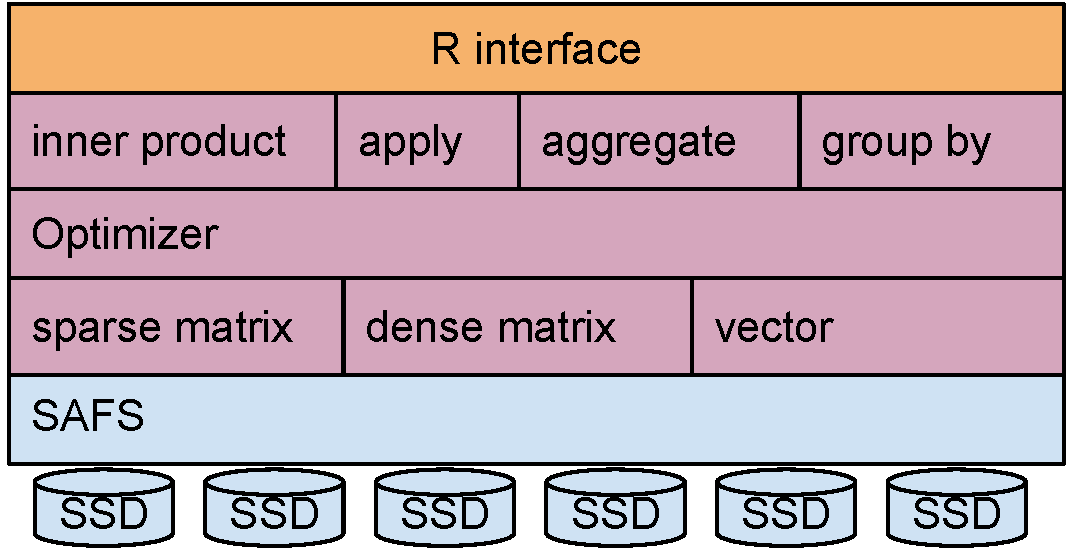
\includegraphics[scale=0.3]{FlashMatrix_figs/architecture.pdf}
\caption{The architecture of FlashR}
\label{fig:arch}
\end{figure}

\subsection{Programming interface}

FlashR provides a matrix-oriented functional programming interface built
on Generalized Operations (GenOps).  GenOps (Table \ref{tbl:genops}) take matrices and
some functions as input and output new matrices that represent computation results.
The input function defines computation on individual elements in input matrices.
GenOps provide a flexible and concise programming interface and, thus,
we focus on optimizing the small set of matrix operations. All of
the GenOps are lazily evaluated to gain performance (Section
\ref{sec:datamove}).

\begin{table}
\begin{center}
\footnotesize
\begin{tabular}{|l|l|l|}
\hline
GenOp & Description \\
\hline
$C=sapply(A, f)$ & $C_{i,j}=f(A_{i,j})$ \\
\hline
$C=mapply(A, B, f)$ & $C_{i,j}=f(A_{i,j}, B_{i,j})$ \\
\hline
$C=mapply.row(A, B, f)$ & $C_{i,j}=f(A_{i,j}, B_j)$ \\
\hline
$C=mapply.col(A, B, f)$ & $C_{i,j}=f(A_{i,j}, B_i)$ \\
\hline
$c=agg(A, f)$ & $c=f(A_{i,j}, c)$, over all $i$, $j$ \\
\hline
$C=agg.row(A, f)$ & $C_i=f(A_{i,j}, C_i)$, over all $j$ \\
\hline
$C=agg.col(A, f)$ & $C_j=f(A_{i,j}, C_j)$, over all $i$ \\
\hline
$C=groupby(A, B, f)$ & $C_{k}=f(A_{i,j}, C_{k})$,\\ & where $B_{i, j}=k$, over all $i,j$ \\
\hline
$C=groupby.row(A, B, f)$ & $C_{k,j}=f(A_{i,j}, C_{k,j})$,\\ & where $B_i=k$, over all $i$ \\
\hline
$C=groupby.col(A, B, f)$ & $C_{i,k}=f(A_{i,j}, C_{i,k})$,\\ & where $B_j=k$, over all $j$ \\
\hline
$C=inner.prod(A, B, f1, f2)$ & $t=f1(A_{i,k}, B_{k,j})$,
\\ & $C_{i,j}=f2(t, C_{i,j})$, over all $k$ \\
\hline
\end{tabular}
\normalsize
\end{center}
\caption{Generalized operations (GenOps) in FlashR.
$A$, $B$ and $C$ are matrices, and $c$ is a scalar.}
\label{tbl:genops}
\end{table}

GenOps are classified into four categories that describe different data access
patterns.
\begin{itemize}
	\item \textbf{Element-wise operations}:
		\textit{sapply} is an element-wise unary operation; \textit{mapply}
		is an element-wise binary operation; \textit{mapply.row} and
		\textit{mapply.col} perform element-wise binary operations on
		the input vector with every row or column of the input matrix
		and output a matrix of the same shape as the input matrix.
	\item \textbf{Aggregation}: \textit{agg} computes aggregation over
		all elements in a matrix and outputs a scalar value; \textit{agg.row}
		computes over all elements in every row and outputs a vector;
		\textit{agg.col} computes over all elements in every column and
		outputs a vector.
	\item \textbf{Groupby}: \textit{groupby} splits the elements of a matrix
		into groups, applies \textit{agg} on each group and outputs a vector;
		\textit{groupby.row} splits rows into groups and applies \textit{agg.col}
		on each group; \textit{groupby.col} splits columns into groups and applies
		\textit{agg.row} on each group. Both \textit{agg.row} and \textit{agg.col}
		output a matrix.
	\item \textbf{inner product} is a generalized matrix multiplication.
		It replaces multiplication and addition in matrix multiplication with
		two functions. Because matrix multiplication is a commonly-used and
		computation-intensive operation, FlashR uses highly optimized matrix
		multiplication implementations to achieve efficiency. For example,
		FlashR uses BLAS for dense floating-point matrices and uses a customized
		matrix multiplication for sparse matrices \cite{SEM_SpMM}.
\end{itemize}

We reimplement a large number of matrix functions in the R \textit{base}
package with the GenOps to provide users a familar programming interface.
Although GenOps provide a set of flexible matrix operations, it is not
the most convenient way to program. Furthermore, by overriding
existing R matrix functions, FlashR scales and parallelizes existing R code
without much modification.
Table \ref{tbl:Rfuns} shows a small subset of R matrix operations and
their implementations with GenOps.

\begin{table}
\begin{center}
\footnotesize
\begin{tabular}{|l|l|l|}
\hline
Function & Implementation with GenOps \\
\hline
$C=A+B$ & $C=mapply(A, B, "+")$ \\
$C=A-B$ & $C=mapply(A, B, "-")$ \\
$C=pmin(A,B)$ & $C=mapply(A, B, "pmin")$ \\
$C=pmax(A,B)$ & $C=mapply(A, B, "pmax")$ \\
$C=sqrt(A)$ & $C=sapply(A, "sqrt")$ \\
$C=abs(A)$ & $C=sapply(A, "abs")$ \\
\hline
$c=sum(A)$ & $c=agg(A, "+")$ \\
$C=rowSums(A)$ & $C=agg.row(A, "+")$ \\
$C=colSums(A)$ & $C=agg.col(A, "+")$ \\
$c=any(A)$ & $c=agg(A, "|")$ \\
$c=all(A)$ & $c=agg(A, "\&")$ \\
\hline
$C=A \%*\% B$ & $C=inner.prod(A, B, "*", "+")$ for integers; \\
 & use BLAS for floating-point values; \\
 & use SpMM \cite{SEM_SpMM} for sparse matrices. \\
\hline
\end{tabular}
\normalsize
\end{center}
\caption{Some of the R matrix functions implemented with GenOps.}
\label{tbl:Rfuns}
\end{table}

In addition to the computation operations, FlashR provides functions for matrix
construction and data access in a FlashR matrix (Table \ref{tbl:utility}). This
includes creating vectors and matrices, loading matrices from external source,
interacting with the R framework, reshape a matrix, access rows and columns of
a matrix and so on.

\begin{table}
\begin{center}
\footnotesize
\begin{tabular}{|l|l|l|}
\hline
Function & Description \\
\hline
$rep.int$ & Create a vector of a repeated value \\
$seq.int$ & Create a vector of sequence numbers \\
$runif.matrix$ & Create a uniformly random matrix  \\
$rnorm.matrix$ & Create a random matrix under a normal distribution \\
\hline
$load.dense.matrix$ & Load a dense matrix to FlashR \\
$load.sparse.matrix$ & Load a sparse matrix to FlashR \\
\hline
$as.matrix$ & Convert a FlashR matrix to an R matrix \\
$fm.as.matrix$ & Convert an R matrix to a FlashR matrix \\
\hline
$t$ & Matrix transpose \\
$rbind$ & Bind matrices by rows \\
$cbind$ & Bind matrices by columns \\
$[]$ & Get rows or columns from a matrix \\
%\hline
%$fm.conv.layout$ & Convert the data layout of a matrix \\
%$fm.set.mate.level$ & Set the materialization level of a \textit{virtual matrix} \\
%$fm.materialize$ & Materialize a \textit{virtual matrix} \\
%$fm.conv.store$ & Move a matrix to a specified storage \\
\hline
\end{tabular}
\normalsize
\end{center}
\caption{Some of the utility functions in FlashR.}
\label{tbl:utility}
\end{table}

The example in Figure \ref{fig:kmeans}(a) illustrates GenOps with k-means
\cite{kmeans}. It first uses \textit{inner.prod} to
compute the Euclidean distance between every data point and every cluster center
and outputs a matrix with each row representing the distances to centers.  
It uses \textit{agg.row} to find the closest
cluster for each data point.  The output matrix 
assigns data points to clusters. It then uses \textit{groupby.row} to count
the number of data points in each cluster and compute the mean of each cluster.

\begin{figure}
\centering
	\footnotesize
	\begin{subfigure}{.25\textwidth}
	\vspace{20pt}
	\centering
	\begin{minted}[mathescape,
	fontsize=\scriptsize,
	frame=single,
	tabsize=2,
	]{R}
# X is the data matrix.
# C is cluster centers.
kmeans.iter <- function(X,C) {
	# Compute pair-wise distance.
	D<-inner.prod(X,t(C),
			"euclidean","+")
	# Find the closest center.
	I<-agg.row(D,"which.min")
	# Count the number of data
	# points in each cluster.
	one<-rep.int(1,nrow(I))
	CNT<-groupby(one,I,"+")
	# Compute the new centers.
	C<-groupby.row(X,I,"+")
	C<-mapply.row(C,CNT,"/")
	list(C=C,I=I)
}
	\end{minted}
	\label{fig:code}
	\caption{R code.}
	\hspace{20pt}
	\end{subfigure}%
	\begin{subfigure}{.25\textwidth}
	\centering
	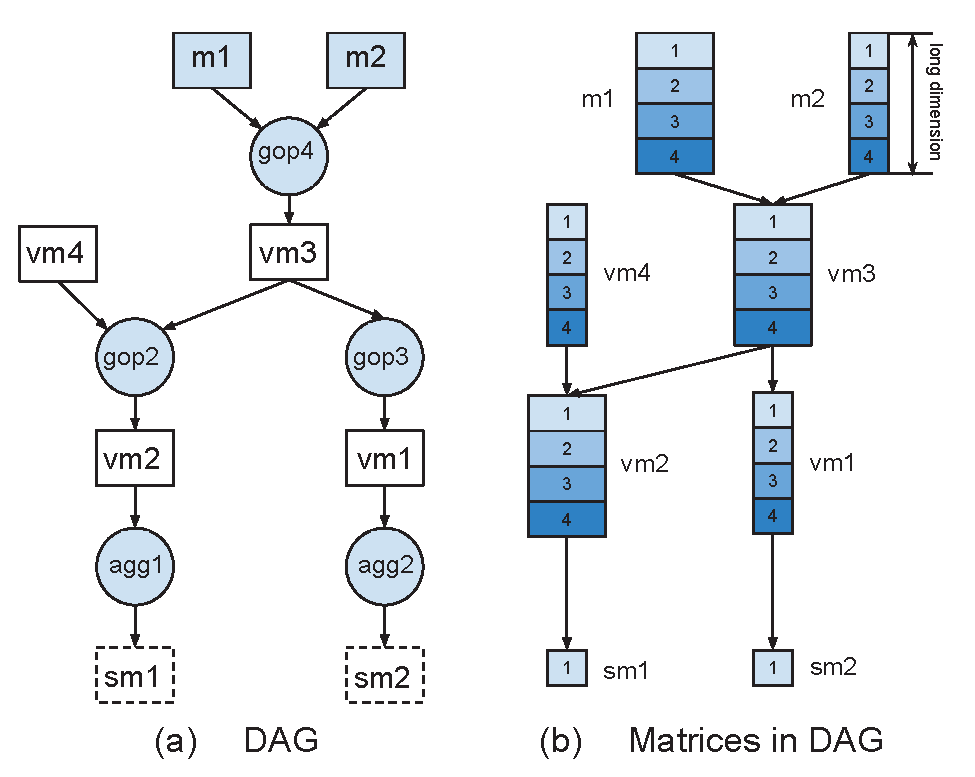
\includegraphics[scale=0.5]{FlashMatrix_figs/DAG.pdf}
	\label{fig:dag}
	\vspace{-4pt}
	\caption{DAG}
	\end{subfigure}
  \vspace{-12pt}
	\caption{k-means implemented with GenOps.}
	\label{fig:kmeans}
  \vspace{-8pt}
\end{figure}

\subsection{Dense matrices}
FlashR optimizes for dense matrices that are rectangular---with
a longer and shorter dimension---because of their frequent occurrence
in machine learning and statistics. Dense matrices can be stored
physically in memory or on SSDs or represented virtually by a sequence of
computations.

\subsubsection{Tall-and-skinny (TAS) matrices}
FlashR optimizes for \textit{tall-and-skinny} (TAS) dense matrices
due to their frequent occurrence in data analysis. These matrices contain
a large number of samples with a relatively few features. Wide-and-short
(WAS) data matrices contain a large number of features with a few samples.
We use similar strategies to optimize wide-and-short matrices. FlashR
supports both row-major and column-major layouts (Figure \ref{fig:den_mat}(a)
and (b)), which allows FlashR to transpose matrices without a copy.
When a TAS matrix is stored in memory, it is stored as an SAFS file
\cite{safs}. We store vectors as a one-column TAS matrix.

\begin{figure}
	\centering
	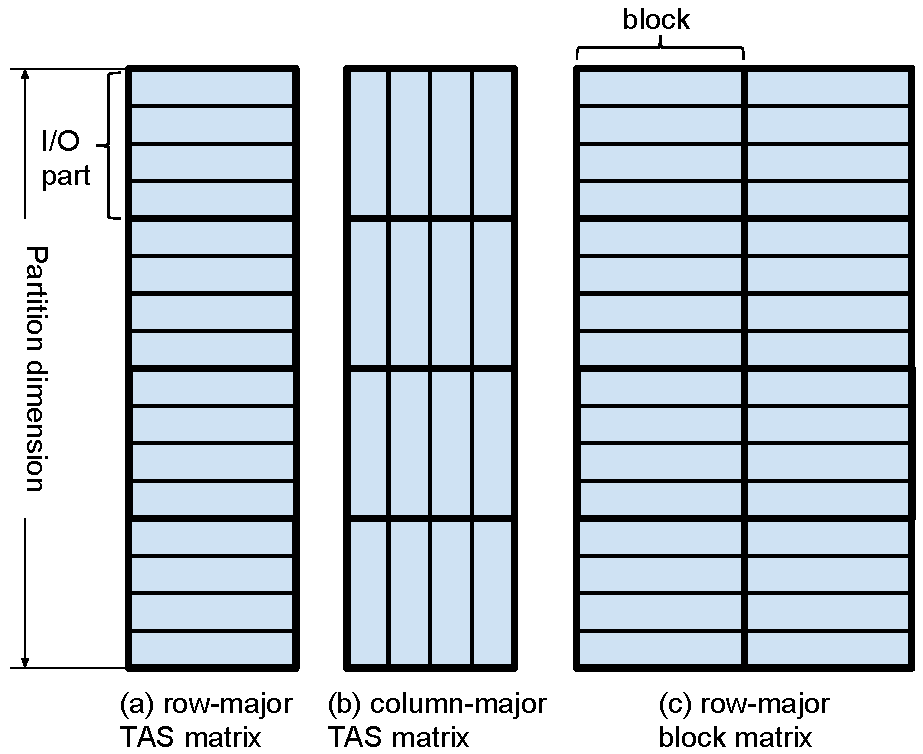
\includegraphics[scale=0.4]{FlashMatrix_figs/dense_matrix2.pdf}
	\caption{The format of a tall dense matrix.}
	\label{fig:den_mat}
  \vspace{-12pt}
\end{figure}

A TAS matrix is partitioned physically into I/O-partitions (Figure
\ref{fig:den_mat}). We refer to the dimension that are partitioned as
\textit{partition dimension}. All elements in an I/O-partition are stored
contiguously regardless of the data layout in the matrix. All 
I/O-partitions have the same number of rows regardless of
the number of columns in a TAS matrix. The number of rows in
an I/O-partition is always $2^i$. This produces column-major TAS
matrices whose data are well aligned in memory to help CPU vectorization.

\subsubsection{Block matrices} \label{sec:block_mat}
FlashR represents a tall matrix as a \textit{block matrix} 
(Figure \ref{fig:den_mat}(c)) comprised of TAS blocks with $32$ columns each,
except the last block. 
Each of the TAS matrices is stored as a separate file on SAFS. 
We decompose a matrix operation
on a block matrix into operations on individual TAS matrices to take advantage
of the optimizations on TAS matrices and reduce data movement.
Coupled with the I/O partitioning on TAS matrices, this strategy enables
2D-partitioning on a dense matrix and each partition fits in main memory.

\dz{Should we explain GenOps on block matrices in more details?}

\subsubsection{Virtual matrices} \label{virt_mat}
To support lazy evaluation, FlashR uses \textit{virtual matrices} that
materialize data on the fly during computation and transfer output as input to
the matrix operation. The data of a matrix are not stored physically.
All GenOps output virtual matrices. A GenOp on a \textit{block matrix} may outputs
a block \textit{virtual matrix}. Virtual matrices are assembled to construct
a directed acyclic graph (DAG) that represents a sequence of matrix computations
(Figure \ref{fig:kmeans}(b)). Virtual matrices are essential to reduce data
movement in the memory hierarchy and memory allocation overhead to accelerate
computation.

\subsubsection{Sink matrices}
The leaf nodes in a DAG are \textit{sink matrices}.
These are produced by aggregation, groupby, and inner product GenOps for which 
the output matrices have a different \textit{partition dimension} size than
the input matrices. \textit{Sink matrices} tend to be small and we store their
results in memory. The maximum size of a sink matrix from an aggregation
is $\sqrt{N}$ for $N$ elements in the input matrix and for groupby
$k \times \sqrt{N}$ for $k$ classes. For most of machine learning and data
analysis tasks, the output of inner product of a wide matrix with a tall matrix
is small because
the long dimension of these matrices is much larger than the short dimension.

%\begin{table}
%\begin{center}
%\footnotesize
%\begin{tabular}{|l|l|l|}
%\hline
%GenOp & Matrix dim & Output size \\
%\hline
%fm.agg & ($n \times p$) & $1$ \\
%\hline
%fm.agg.row & ($n \times p$), $n < p$ & $n$ \\
%\hline
%fm.agg.col & ($n \times p$), $n > p$ & $p$ \\
%\hline
%fm.groupby.row & ($n \times p$), $n > p$ & $p \times k$ \\
%\hline
%fm.groupby.col & ($n \times p$), $n < p$ & $n \times k$ \\
%\hline
%fm.inner.prod & ($p1 \times n$) $\times$ ($n \times p2$), & $p1 \times p2$ \\
%			  & $n \gg p1, n \gg p2$ &  \\
%\hline
%\end{tabular}
%\normalsize
%\end{center}
%\caption{GenOps that output \textit{sink matrices}.}
%\label{tbl:sink}
%\end{table}

\subsection{Sparse matrices}
FlashR supports sparse matrices and mainly optimizes for matrix multiplication
on sparse matrices.
For large sparse matrices that arise from graphs (e.g., social networks
and Web graphs), which has a large number of rows and columns, FlashR integrates
with an efficient implementation \cite{SEM_SpMM} that stores sparse matrices
in a compact format on SSDs and performs matrix multiplication on such sparse
matrices in semi-external memory, i.e., we keep the sparse matrix on SSDs and
the dense matrix or part of the dense matrix in memory.
For sparse matrices with many rows and few columns or with many columns
and few rows, FlashR stores the sparse matrices with the coordinate format
(COO). These rectangular sparse matrices usually require small memory storage,
so the current implementation keeps them in memory.

\subsection{Reducing data movement}\label{sec:datamove}
To optimize evaluation, FlashR lazily evaluates matrix operations and
constructs one or more directed-acyclic graphs (DAGs) connecting GenOps and
matrices. Figure \ref{fig:kmeans} (b) shows the DAG for k-means.
Then it performs all computation in a DAG together 
to minimize data movement in the memory hierarchy.
This data-driven, lazy evaluation allows out-of-core problems 
to approach in-memory performance.

\subsubsection{Directed-acyclic graphs (DAGs)}
A DAG comprises a set of matrix nodes (rectangles) and computation nodes
(ellipses). The majority of matrix nodes are virtual matrices (dashed line rectangles).
For k-means, only the input matrix \textit{X} has materialized data.
A computation node references a GenOp and input matrices and
may contain some immutable computation state, such as scalar variables and
small matrices. 

FlashR grows each DAG as large as possible, by allowing virtual matrices
of different shapes in a DAG, to increase the ratio of computation to I/O
(Figure \ref{fig:mater}). To simplify evaluation and data flow, 
all virtual matrices in internal matrix nodes need to have the same
\textit{partition dimension} size. \textit{Sink matrices} are edge nodes
in the DAG because they have different \textit{partition dimension} sizes
from the internal matrices. Any computation that uses these
\textit{sink matrices} cannot be connected to the same DAG.  

\subsubsection{DAG materialization}
FlashR allows both explicit and implicit DAG materialization.
We materialize virtual matrices that access the same set of dense matrices
stored on SSDs together. To explicitly
materialize a DAG, a user can invoke \textit{fm.materialize} to materialize
\dz{more explanation}

Access to elements of a \textit{sink matrix} (leaf node) triggers materialization
of the entire DAG where the \textit{sink matrix} connects to. As such,
FlashR does not require explicit materialization from users in most cases
to further simplifies programming. By default,
FlashR saves the computation results of all \textit{sink matrices} of
the DAG in memory and discard the data of non-\textit{sink matrices} on the fly.
Because \textit{sink matrices} tend to be small, this materialization
rule leads to small memory consumption.
In exceptional cases, especially for iterative algorithms,
it is helpful to save some non-\textit{sink matrices} to avoid
redundant computation and I/O across iterations.  We allow users to
set a flag on any matrix to materialize and cache data in memory
or on SSDs during computation, similar to caching an RDD in Spark.

\begin{figure}
	\centering
	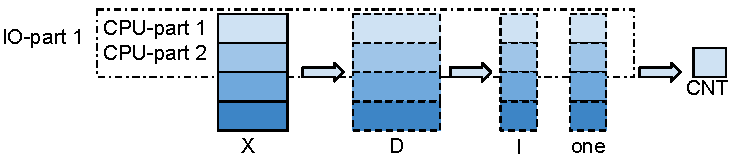
\includegraphics[scale=0.6]{FlashMatrix_figs/materialize.pdf}
  \vspace{-4pt}
	\caption{Materializing matrix partitions in a DAG.}
	\label{fig:mater}
  \vspace{-8pt}
\end{figure}

During DAG materialization, FlashR partitions matrices in a DAG and
materializes partitions separately
(Figure \ref{fig:mater}). This is possible because all matrices, except
sink matrices, share the same partition dimension. 
A partition $i$ of a virtual matrix requires data only from partitions
$i$ of the parent matrices.  All DAG operations in a partition are processed by 
the same thread to minimize remote memory accesses in a NUMA machine.
When materializing a sink matrix, each thread computes partial
aggregation results on the partitions assigned to the thread. 
Then, FlashR merges per-thread partial results to construct the output.

FlashR uses two-level partitioning on dense matrices to reduce data
movement between SSDs and CPU. It assigns I/O-partitions to a thread as
a parallel task.
%A small partition size (\rb{How?}) balances the overhead of accessing a partition,
%computation, skew, and memory consumption. 
It further splits I/O-partitions into processor cache (Pcache)
partitions at run time.  Each thread materializes one Pcache-partition
at a time. Matrix operations run on TAS matrices or block matrices that are
divided into TAS matrices so that a Pcache-partition fits in the CPU L1/L2 cache.
Figure \ref{fig:mater} shows recursive materialization.
Matrix \textit{CNT} triggers materialization of
Pcache-partitions of \textit{I} and \textit{one}, which in turn triggers 
partitions of \textit{D}, and so on. Eventually, the process triggers data access
to an I/O-partition of input matrix \textit{X} from SSDs. 

FlashR takes efforts to increase hits in the CPU cache, which 
significantly reduces data movement between CPU and memory.
When materializing output to a virtual matrix, the thread passes
the output as input to the subsequent
GenOp, instead of materializing the next Pcache-partition.
This ensures that a Pcache-partition resides in the CPU cache
when the next GenOp consumes it. 
In each thread, all intermediate matrices have only one 
Pcache-partition materialized
at any time to reduce CPU cache pollution.
%To reduce CPU cache polution, a CPU-level partition is discarded once it is
%used by all children matrices.

%materialization on block matrices.

%In a DAG, a matrix may be
%required by multiple GenOps. As such, each matrix always buffers one materialized
%CPU-level partition in each thread to avoid redundant computation.

% TODO
%To keep data in CPU cache as long as possible, we reuse the memory buffers
%to reduce the number of memory buffers used in the computation and avoid CPU
%cache polution.

\subsection{Parallel execution and I/O access}
FlashR dispatches computation to threads so that they
issue large reads and writes to SSDs, while still achieving good load balancing.
FlashR uses a global task scheduler to assign I/O-partitions to threads
dynamically. Initially, the scheduler assigns multiple contiguous I/O-partitions
to a thread. The thread reads these in a single large I/O.
The number of contiguous I/O-partitions assigned to a thread is determined by
the block size of SAFS.
As the computation nears an end, the scheduler dispatches single I/O-partitions. 
% DZTODO -- "always is wrong"  -- consider out of order execution
%The scheduler always ensures that all threads are working on I/O-partitions that are adjacent to
%each other on storage.
The scheduler dispatches I/O-partitions sequentially to maximize contiguity in memory
and on SSD.
When the DAG stores the materialized result of a non-\textit{sink matrix}, 
contiguity makes it easier for the file system to merge
writes from multiple threads, which helps to sustain write throughout and reduces
write amplification \cite{ripq}.

%For a block matrix with many TAS matrices, we parallelize the computation and
%I/O access differently. One of the goals is to reduce memory consumption.
%Instead of getting the row/column range from all TAS matrices before performing
%computation, we read the row/column range from some TAS matrices first, perform
%computation and move on to the next TAS matrices in the same range. This is
%very helpful if the computation is aggregation.

\section{Machine learning algorithms and implementations}

\begin{figure}
\centering
	\footnotesize
	\centering
	\begin{minted}[mathescape,
	fontsize=\scriptsize,
	frame=single,
	tabsize=2,
	]{R}
pagerank <- function(graph, d=0.15, epsilon=1e-2) {
	N <- nrow(graph)
	pr1 <- fm.rep.int(1/N, N)
	out.deg <- graph %*% fm.rep.int(1, N)
	converge <- 0
	graph <- t(graph)
	while (converge < N) {
		pr2 <- (1-d)/N+d*(graph %*% (pr1/out.deg))
		diff <- abs(pr1-pr2)
		converge <- sum(diff < epsilon)
		pr1 <- pr2
	}
	pr1
}
	\end{minted}
	\label{fig:code}
	\caption{k-means implemented with GenOps.}
	\label{fig:kmeans}
  \vspace{-8pt}
\end{figure}
